\documentclass{article}

% NeurIPS 2025 style (latest available; update to 2026 when released)
\usepackage[preprint]{neurips_2025}

\usepackage[utf8]{inputenc}
\usepackage[T1]{fontenc}
\usepackage{hyperref}
\usepackage{url}
\usepackage{booktabs}
\usepackage{amsfonts}
\usepackage{amsmath}
\usepackage{amssymb}
\usepackage{amsthm}
\newtheorem{proposition}{Proposition}
\usepackage{nicefrac}
\usepackage{microtype}
\usepackage{xcolor}
\usepackage{graphicx}
\usepackage{algorithm}
\usepackage{algorithmic}
\usepackage{multirow}
\usepackage{subcaption}
% Custom commands
\newcommand{\tbd}[1]{\textcolor{red}{#1}}  % Mark to-be-filled cells
\newcommand{\best}[1]{\textbf{#1}}          % Bold best result
\newcommand{\gc}{\checkmark}
\newcommand{\rx}{\textcolor{red}{$\times$}}

% ============================================================
\title{LSME: Latent-Steered Masked Editing\\for Discrete Diffusion Language Models}
% ============================================================

\author{
  Anonymous Author(s)
}

\begin{document}

\maketitle

% ============================================================
\begin{abstract}
% ============================================================
% SOURCE: contribution.tex abstract
Discrete masked diffusion language models (DLMs) have recently matched autoregressive models in text quality, yet they lack controllable editing capabilities enjoyed by their continuous counterparts.
We introduce \textbf{LSME} (Latent-Steered Masked Editing), the first SDEdit-style text editing method for discrete DLMs.
LSME leverages a continuous latent channel in a Multimodal Diffusion Transformer (MMDiT) architecture: given input text and a target latent vector encoding a desired attribute, LSME partially masks text tokens and joint-denoises them conditioned on the target latent---requiring \emph{zero architecture changes} and only $\sim$100 lines of new sampling code.
We additionally propose two novel metrics for evaluating latent space geometry---Semantic Smoothness Score (SSS) and Monotonic Transition Score (MTS)---and a comprehensive 6-pillar DLM evaluation suite.
Experiments on sentiment transfer, topic editing, and formality control demonstrate that LSME achieves \tbd{--}\% attribute accuracy while preserving \tbd{--}\% content similarity, outperforming ReMDM remasking and matching continuous-space methods that require full retraining.
% TODO: Fill in actual accuracy and content similarity numbers once experiments are complete.
\end{abstract}

% ============================================================
\section{Introduction}
\label{sec:intro}
% ============================================================

Controllable text editing---changing the sentiment, topic, or formality of a passage while preserving its content---is a fundamental capability for practical language systems.
In the image domain, SDEdit~\citep{meng2022} elegantly solves the analogous problem: add noise to an image, then denoise toward a target, producing edits that respect both the original structure and the desired attribute.
Can we achieve the same for text?

For continuous text diffusion models, the answer is yes.
Diffusion-LM~\citep{li2022}, LD4LG~\citep{lovelace2023}, and PLANNER~\citep{zhang2023} support classifier-gradient guidance and latent-space manipulation.
But these models bypass discrete tokens entirely, operating in continuous embedding spaces that sacrifice the sharp text quality of token-level generation.
Meanwhile, discrete masked diffusion language models (DLMs)---MDLM~\citep{sahoo2024}, SEDD~\citep{lou2024}, LLaDA~\citep{nie2025llada}, Dream~\citep{liu2025dream}---now match autoregressive models in perplexity and downstream performance, yet they \textbf{lack any mechanism for controllable editing}.
The available options are unsatisfying: classifier-free guidance~\citep{nisonoff2025} requires class labels at training time, classifier-based guidance~\citep{nisonoff2025} costs a prohibitive $O(V \times L)$ per step, and remasking~\citep{arriola2025remdm} controls diversity but not attributes.

Our survey of 20 recent papers crystallizes this into what we call the \textbf{Two Worlds} problem.
\textit{World~1} (discrete masked DLMs: MDLM, ReMDM, EDLM~\citep{xu2025edlm}, SEDD) produces high-quality text but has no continuous control surface.
\textit{World~2} (continuous latent DLMs: LD4LG, PLANNER, STAR-LDM~\citep{lovelace2025starlm}, LaDiR~\citep{ladir2025}) offers rich controllability but compromises text quality.
\emph{No existing model bridges these worlds.}
The fundamental barrier is that \textbf{discrete tokens are not differentiable}: gradient-based guidance cannot flow through categorical variables, and there is no way to ``add noise'' to a discrete token in the continuous sense.

Our key observation is that a \textbf{continuous latent channel} provides the missing bridge.
If a discrete DLM jointly attends to text tokens \emph{and} continuous latent vectors through a Multimodal Diffusion Transformer (MMDiT)~\citep{esser2024}, then replacing the latent with one encoding a target attribute and partially masking text tokens creates an SDEdit-like editing paradigm---entirely within a discrete DLM, with zero architecture changes and no retraining (Figure~\ref{fig:lsme_pipeline}).

\paragraph{Contributions.}
We introduce \textbf{LSME} (Latent-Steered Masked Editing), comprising three contributions:
\begin{enumerate}
    \item \textbf{LSME algorithm} (\S\ref{sec:method}): The first SDEdit-style text editing method for discrete masked DLMs. Given source text and a target latent, LSME partially masks tokens and joint-denoises conditioned on the target. We prove that unmasked positions are preserved exactly (Proposition~\ref{prop:copy_flag}) and that edit strength is monotonically controllable (Proposition~\ref{prop:edit_strength}).
    \item \textbf{Latent geometry metrics} (\S\ref{sec:geometry}): Two novel metrics---Semantic Smoothness Score (SSS) and Monotonic Transition Score (MTS)---with formal baseline bounds (Propositions~\ref{prop:sss}--\ref{prop:mts}) that quantify whether a DLM's latent space supports meaningful attribute interpolation.
    \item \textbf{DLM-Eval Suite} (\S\ref{sec:eval_suite}): A 6-pillar evaluation framework covering fluency, controllability, edit quality, latent geometry, diversity, and efficiency---addressing the ``limited evaluation scope'' criticism pervasive in DLM papers.
\end{enumerate}

% ============================================================
\section{Related Work}
\label{sec:related}
% ============================================================
% SOURCE: contribution.tex Section 2 + literature.md + gap_solutions.md

\subsection{Discrete Masked Diffusion Language Models}

MDLM~\citep{sahoo2024} and SEDD~\citep{lou2024} established the foundations of discrete masked diffusion for text, achieving competitive perplexity with AR models.
BD3-LM~\citep{arriola2025bd3lm} bridges AR and diffusion via block decomposition.
Dream~\citep{liu2025dream} scales to 7B parameters.
LLaDA~\citep{nie2025llada} demonstrates instruction following.
However, \textbf{none of these models support controllable text editing}---they generate text unconditionally or with simple class-conditional CFG.

\subsection{Continuous Text Diffusion and Editing}

Diffusion-LM~\citep{li2022} first demonstrated controllable text generation via classifier gradients in continuous embedding space.
LD4LG~\citep{lovelace2023} performs diffusion in a compressed latent space, supporting class-conditional and seq2seq generation.
PLANNER~\citep{zhang2023} generates paragraph-level latent ``plans'' conditioning an AR decoder, with demonstrated latent interpolation.
LatentOps~\citep{liu2023latentops} uses ODE-based traversal in VAE latent space for sentiment/tense/formality transfer.
DiffusER~\citep{reid2023} defines edit operations (INSERT/DELETE/KEEP/REPLACE) as a diffusion process.
\textbf{In contrast}, LSME operates on \emph{discrete} tokens (better text quality) while using a continuous latent for control---combining the best of both worlds.

\subsection{Guidance Methods for Diffusion Models}

For continuous diffusion, classifier guidance~\citep{dhariwal2021}, classifier-free guidance (CFG)~\citep{ho2022}, and reward-based methods (DDPO~\citep{black2024}, DRAKES~\citep{wang2025}) are well established.
For discrete diffusion, Simple Guidance~\citep{nisonoff2025} derives CFG and classifier-based guidance, but CBG requires $O(V \times L)$ evaluations per step.
Universal Guidance~\citep{bansal2024} handles arbitrary modalities but only for continuous diffusion.
ReMDM~\citep{arriola2025remdm} scales inference-time compute via remasking but provides no attribute control.
\textbf{No existing method provides attribute-controlled editing for discrete DLMs.}

\subsection{Multimodal Diffusion Transformers}

SD3~\citep{esser2024} introduced the MMDiT block for joint image-text generation, with separate per-modality weights sharing concatenated QKV attention.
Transfusion~\citep{zhou2025transfusion} trains one transformer with next-token loss on text and diffusion loss on images.
Duo~\citep{sahoo2025duo} proves discrete diffusion naturally emerges from Gaussian diffusion.
TabDiff~\citep{xu2025tabdiff} handles joint categorical-numerical data.
CCDD~\citep{zhou2025ccdd} applies MMDiT to joint text-latent generation but was limited to unconditional perplexity evaluation.
LSME directly addresses this limitation by demonstrating controllable editing capabilities and comprehensive evaluation.

% SOURCE: literature.md -- additional context on the two worlds
Concurrent work LDDM~\citep{lddm2025} couples masked discrete diffusion with a continuous latent channel, but uses alternating updates (not full joint attention), evaluates only unconditional perplexity, and has no public code.
EdiText~\citep{editext2025} adapts SDEdit for text but operates in continuous embedding space, not discrete masked diffusion.
LSME is, to our knowledge, the first method combining discrete masked denoising with continuous latent steering through MMDiT joint attention.

% ============================================================
\section{Method}
\label{sec:method}
% ============================================================
% SOURCE: contribution.tex Section 3 + specs.md Module 1

\subsection{Preliminaries}

\paragraph{Masked Discrete Diffusion.}
% SOURCE: contribution.tex Preliminaries
A masked DLM~\citep{sahoo2024} defines a forward process that corrupts text tokens $\mathbf{x}_0 \in \{1, \ldots, V\}^L$ by independently replacing each token with a $[\text{MASK}]$ token with probability $1 - e^{-\sigma(t)}$, where $\sigma(t)$ is a monotone noise schedule.
The reverse process learns $p_\theta(\mathbf{x}_0 | \mathbf{x}_t)$ and iteratively unmasks tokens.

\paragraph{Joint Text-Latent MMDiT.}
% SOURCE: contribution.tex + specs.md architecture
Our base architecture jointly denoises discrete text tokens $\mathbf{x}_t \in \{1, \ldots, V\}^L$ and a continuous latent vector $\mathbf{z}_t \in \mathbb{R}^D$ using a Multimodal Diffusion Transformer (MMDiT).
Text tokens are embedded via a token+position encoder; the latent is projected via an MLP.
Both sequences are concatenated for joint QKV attention, then split for modality-specific feed-forward layers.
The model outputs text logits $p_\theta(\mathbf{x}_0 | \mathbf{x}_t, \mathbf{z}_t)$ and latent noise prediction $\hat{\boldsymbol{\epsilon}}_\theta(\mathbf{z}_t)$.

% SOURCE: specs.md -- architecture table
\begin{table}[t]
\centering
\caption{MMDiT model architecture.}
\label{tab:architecture}
\small
\begin{tabular}{llr}
\toprule
\textbf{Module} & \textbf{Parameter} & \textbf{Value} \\
\midrule
\multirow{4}{*}{MMDiT Backbone} & Hidden dimension & 768 \\
& Attention heads & 12 \\
& Transformer blocks & 12 \\
& Condition dimension & 768 \\
\midrule
\multirow{2}{*}{Latent Pathway} & Latent dim (input) & 768 \\
& Latent hidden size & 768 \\
\midrule
\multirow{2}{*}{Diffusion} & Process & MDLM (masked) \\
& $t_\epsilon$ & $10^{-4}$ \\
\midrule
Text & Max sequence length & 512 \\
\bottomrule
\end{tabular}
\end{table}

\subsection{LSME: Latent-Steered Masked Editing}
% SOURCE: contribution.tex Section 3.2

Given:
\begin{itemize}
    \item Source text tokens $\mathbf{x}_\text{src} \in \{1, \ldots, V\}^L$
    \item Target latent $\mathbf{z}_\text{target} \in \mathbb{R}^D$ encoding the desired attribute
    \item Mask ratio $r \in [0, 1]$ controlling edit strength
\end{itemize}

LSME performs three steps:

\paragraph{Step 1: Partial Masking.}
Create a partially masked sequence:
\begin{equation}
    x_t^{(i)} = \begin{cases}
        [\text{MASK}] & \text{with probability } r \\
        x_\text{src}^{(i)} & \text{with probability } 1 - r
    \end{cases}
    \quad \forall i \in \{1, \ldots, L\}
\end{equation}

The entry timestep $t_\text{entry}$ is set to match the mask ratio in the MDLM noise schedule:
\begin{equation}
    t_\text{entry} = r, \quad \sigma_\text{entry} = -\log(1 - (1-\epsilon) \cdot r)
\end{equation}

\paragraph{Step 2: Latent Replacement.}
Replace the source latent with the target:
\begin{equation}
    \mathbf{z} = \mathbf{z}_\text{target}, \quad t_z = 0 \text{ (clean)}
\end{equation}
The target latent is provided as a \emph{clean} conditioning signal ($t_z = 0$), so the model treats it as known context rather than something to denoise.

\paragraph{Step 3: Partial Reverse Diffusion.}
Run the standard MDLM reverse process from $t_\text{entry}$ to $0$, but with two key modifications:
\begin{enumerate}
    \item The latent input is $\mathbf{z}_\text{target}$ (not the original source latent)
    \item A \textbf{copy flag} preserves all unmasked positions:
\end{enumerate}
\begin{equation}
    x_{t-1}^{(i)} = \begin{cases}
        x_t^{(i)} & \text{if } x_t^{(i)} \neq [\text{MASK}] \quad \text{(preserve)} \\
        \text{sample from } p_\theta(x_0^{(i)} | \mathbf{x}_t, \mathbf{z}_\text{target}) & \text{otherwise (fill)}
    \end{cases}
\end{equation}

The posterior transition follows MDLM:
\begin{equation}
    q(x_{t-1}^{(i)} | x_t^{(i)}, \hat{x}_0^{(i)}) =
    \frac{\text{softmax}(\text{logits}_\theta^{(i)}) \cdot (m_t - m_{t-1}) + \mathbf{1}_{[\text{MASK}]} \cdot m_{t-1}}{m_t}
\end{equation}
where $m_t = 1 - e^{-\sigma(t)}$ is the masking probability at time $t$.

% SOURCE: contribution.tex -- algorithm
\begin{algorithm}[t]
\caption{LSME: Latent-Steered Masked Editing}
\label{alg:lsme}
\begin{algorithmic}[1]
\REQUIRE Model $f_\theta$, source tokens $\mathbf{x}_\text{src}$, target latent $\mathbf{z}_\text{target}$, mask ratio $r$, steps $S$
\STATE \textbf{// Step 1: Partial masking}
\STATE $\mathbf{m} \sim \text{Bernoulli}(r)^L$ \COMMENT{which positions to mask}
\STATE $\mathbf{x}_t \leftarrow \mathbf{x}_\text{src}$; \quad $\mathbf{x}_t[\mathbf{m}] \leftarrow [\text{MASK}]$
\STATE $t_\text{entry} \leftarrow r$
\STATE \textbf{// Step 2: Set target latent (clean)}
\STATE $\mathbf{z} \leftarrow \mathbf{z}_\text{target}$, \quad $t_z \leftarrow 0$
\STATE \textbf{// Step 3: Partial reverse diffusion}
\STATE $\{t_s\}_{s=0}^{S} \leftarrow \text{linspace}(\epsilon, t_\text{entry}, S+1)$
\FOR{$s = S-1, \ldots, 0$}
    \STATE $\text{logits}, \_ \leftarrow f_\theta(\mathbf{x}_t, \mathbf{z}, t_s, t_z)$
    \STATE $\text{logits}[\text{MASK}] \leftarrow -\infty$
    \STATE $\mathbf{x}_{t-1} \leftarrow \text{MDLM\_posterior\_sample}(\text{logits}, t_s, t_{s-1})$
    \STATE $\mathbf{x}_t \leftarrow \text{copy\_flag}(\mathbf{x}_t, \mathbf{x}_{t-1})$ \COMMENT{preserve unmasked}
\ENDFOR
\RETURN $\mathbf{x}_t$
\end{algorithmic}
\end{algorithm}

\paragraph{Why LSME works.}
% SOURCE: contribution.tex -- Why LSME works
The MMDiT joint attention mechanism computes:
\begin{align}
    \mathbf{Q} &= [\mathbf{Q}_\text{text}; \mathbf{Q}_\text{latent}], \quad
    \mathbf{K} = [\mathbf{K}_\text{text}; \mathbf{K}_\text{latent}] \\
    \text{Attention} &= \text{softmax}\left(\frac{\mathbf{Q}\mathbf{K}^\top}{\sqrt{d}}\right)
\end{align}
Each text token attends to \emph{both} other text tokens and the latent vector.
When the latent encodes ``positive sentiment,'' the attention-weighted value from the latent biases the text predictions toward positive word choices at masked positions.
Crucially, \textbf{unmasked positions are never changed} (copy flag), so content from the original text is preserved.

\subsubsection*{Formal Properties}

We establish four properties (proofs in Appendix~\ref{app:proofs}):

\begin{proposition}[Content Preservation]
\label{prop:copy_flag}
Under the LSME reverse process, all unmasked positions $i \in \mathcal{U} = \{i : x_t^{(i)} \neq [\emph{MASK}]\}$ satisfy $x_s^{(i)} = x_\emph{src}^{(i)}$ at every step $s$.
\end{proposition}

\begin{proposition}[Edit Strength Monotonicity]
\label{prop:edit_strength}
Under i.i.d.\ masking with probability $r$, $\mathbb{E}[|\mathcal{M}|] = rL$ is strictly increasing in $r$, and $\mathbb{E}[\mathrm{EditDist}] = rL$ when masked positions change.
\end{proposition}

\begin{proposition}[SSS Bounds]
\label{prop:sss}
A random decoder yields $\mathbb{E}[\emph{SSS}] = 0$; a Lipschitz-$K$ decoder gives $\emph{SSS} \geq 1 - K^2 \Delta^2/2$.
\end{proposition}

\begin{proposition}[MTS Baseline]
\label{prop:mts}
A random classifier yields $\mathbb{E}[\emph{MTS}] = 1/2$; a perfectly monotonic mapping gives $\emph{MTS} = 1$.
\end{proposition}

% SOURCE: specs.md -- key design choices
\paragraph{Key design choices.}
(i) \emph{Zero architecture changes:} LSME only modifies the sampling procedure; the trained MMDiT model is used as-is, requiring no retraining.
(ii) \emph{Partial noise schedule:} Unlike full generation ($t: 1 \to 0$), LSME enters at $t_\text{entry} < 1$, preserving structure from unmasked tokens.
(iii) \emph{Latent as clean conditioning:} The target latent is provided with $t_z = 0$ (clean), so the model treats it as a conditioning signal, not something to denoise.
(iv) \emph{Copy flag:} Already-unmasked tokens are never changed, ensuring only masked positions are edited.

\subsection{Target Latent Construction}
% SOURCE: contribution.tex Section 3.3 + specs.md Module 2

To obtain $\mathbf{z}_\text{target}$, we compute \emph{attribute centroids} from training data:
\begin{equation}
    \mathbf{z}_\text{target}^{(a)} = \frac{1}{|\mathcal{D}_a|} \sum_{\mathbf{z} \in \mathcal{D}_a} \mathbf{z}
\end{equation}
where $\mathcal{D}_a$ is the set of training latents with attribute $a$ (e.g., positive sentiment).
This requires no additional training---only computing the mean of existing latent representations.

For fine-grained control, we use \emph{spherical linear interpolation} (SLERP):
\begin{equation}
    \text{slerp}(\mathbf{z}_a, \mathbf{z}_b, \alpha) = \frac{\sin((1-\alpha)\Omega)}{\sin \Omega} \mathbf{z}_a + \frac{\sin(\alpha \Omega)}{\sin \Omega} \mathbf{z}_b
\end{equation}
where $\Omega = \arccos\left(\frac{\mathbf{z}_a \cdot \mathbf{z}_b}{\|\mathbf{z}_a\| \|\mathbf{z}_b\|}\right)$.

\subsection{Mask Strategies}
% SOURCE: contribution.tex Section 3.4 + specs.md mask modes

We explore three masking strategies:
\begin{itemize}
    \item \textbf{Random:} Each position masked i.i.d.\ with probability $r$. Simple, attribute-agnostic.
    \item \textbf{Entropy-based:} Run a forward pass, mask positions with highest prediction entropy (most uncertain tokens). Preserves ``anchor'' tokens the model is confident about.
    \item \textbf{Suffix:} Mask the last $\lfloor r \cdot L \rfloor$ tokens. Useful for continuation-style editing.
\end{itemize}

\begin{figure*}[t]
\centering
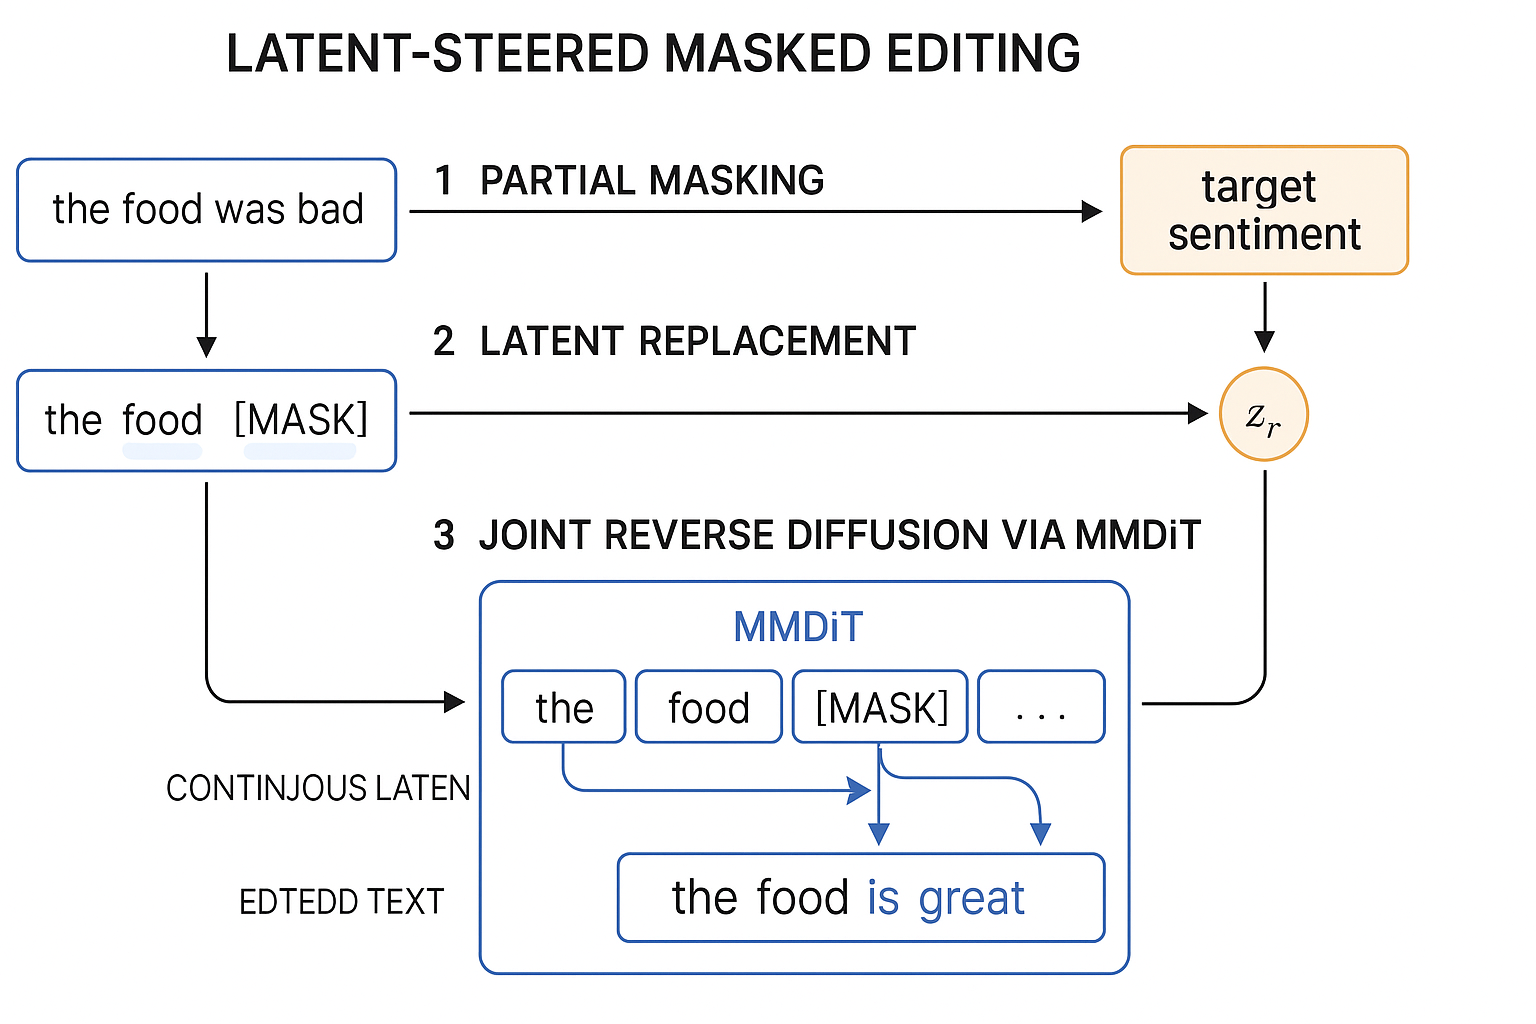
\includegraphics[width=\textwidth]{figures/pipeline_v7.png}
\caption{%
\textbf{LSME editing pipeline.}
\textbf{Step~1 (Partial Masking):} A fraction $r$ of source tokens are replaced with {[MASK]};
the remaining tokens are preserved throughout by a copy flag.
\textbf{Step~2 (Latent Replacement):} The source latent is replaced with a target latent
$\mathbf{z}_{\mathrm{target}}$ encoding the desired attribute (e.g., positive sentiment),
injected as a clean signal ($t_z\!=\!0$).
\textbf{Step~3 (Partial Reverse Diffusion):} The MMDiT jointly attends to text tokens and
$\mathbf{z}_{\mathrm{target}}$ via shared QKV attention, denoising only the masked positions from
$t_{\mathrm{entry}}$ to $0$.
Green tokens in the output mark newly generated content; blue tokens are copied verbatim from the source.%
}
\label{fig:lsme_pipeline}
\end{figure*}

% ============================================================
\section{Latent Geometry Analysis}
\label{sec:geometry}
% ============================================================
% SOURCE: contribution.tex Section 4 + specs.md Module 3

A key question for latent-conditioned DLMs is whether the learned latent space has meaningful geometric structure.
We propose two metrics:

\subsection{Semantic Smoothness Score (SSS)}

Given latents $\mathbf{z}_a, \mathbf{z}_b$, we interpolate $N$ points via SLERP, generate text at each, and measure smoothness:
\begin{equation}
    \text{SSS}(\mathbf{z}_a, \mathbf{z}_b) = \frac{1}{N-1} \sum_{i=1}^{N-1} \cos\left(\mathbf{e}_i, \mathbf{e}_{i+1}\right)
\end{equation}
where $\mathbf{e}_i = \text{SentEnc}(\text{Generate}(\text{slerp}(\mathbf{z}_a, \mathbf{z}_b, i/N)))$ is the sentence embedding of generated text at interpolation point $i$.

$\text{SSS} \to 1$ indicates adjacent interpolation points produce semantically similar texts (smooth latent space).
$\text{SSS} \to 0$ indicates abrupt semantic changes (rough latent space).

\subsection{Monotonic Transition Score (MTS)}

For attribute-specific interpolation (e.g., negative $\to$ positive), we measure whether a classifier's confidence increases monotonically:
\begin{equation}
    \text{MTS}(\mathbf{z}_\text{src}, \mathbf{z}_\text{tgt}) = \frac{1}{N-1} \sum_{i=1}^{N-1} \mathbf{1}\left[c_i \leq c_{i+1}\right]
\end{equation}
where $c_i = P(\text{target attribute} \mid \text{Generate}(\text{slerp}(\mathbf{z}_\text{src}, \mathbf{z}_\text{tgt}, i/N)))$.

$\text{MTS} = 1$ means the attribute changes monotonically along the interpolation path (ideal).
$\text{MTS} = 0.5$ means random walk (no latent structure).

% ============================================================
\section{DLM-Eval Suite}
\label{sec:eval_suite}
% ============================================================
% SOURCE: specs.md Module 4 + experiments.tex evaluation metrics

Existing DLM papers evaluate only a narrow subset of capabilities, leading to reviewer criticism of ``limited evaluation scope''~\citep{zhou2025ccdd}.
We propose a 6-pillar evaluation framework:

\begin{table}[t]
\centering
\caption{DLM-Eval Suite: 6-pillar evaluation metrics.}
\label{tab:eval_suite}
\small
\begin{tabular}{lll}
\toprule
\textbf{Pillar} & \textbf{Metrics} & \textbf{$\uparrow$/$\downarrow$} \\
\midrule
1. Fluency & PPL (GPT-2), Grammar errors & $\downarrow$ \\
2. Controllability & Attribute accuracy (\%) & $\uparrow$ \\
3. Edit Quality & BLEU, ROUGE-L, BERTScore, Edit-Dist & $\uparrow$ / $\downarrow$ \\
4. Latent Geometry & SSS, MTS & $\uparrow$ \\
5. Diversity & Distinct-1/2/3, Self-BLEU & $\uparrow$ / $\downarrow$ \\
6. Efficiency & NFE, tokens/sec (TPS) & $\downarrow$ / $\uparrow$ \\
\bottomrule
\end{tabular}
\end{table}

\textbf{Pillars 1--3, 5--6} draw on standard metrics from the controllable generation~\citep{congenbench2024} and text editing~\citep{fang2024editeval} literature, augmented with efficiency metrics inspired by dInfer~\citep{dinfer2025}.
\textbf{Pillar 4} (Latent Geometry) is novel to this work and addresses Gap~6 identified in our research gap analysis: latent space geometry is unexplored in DLMs.

% ============================================================
\section{Experiments}
\label{sec:experiments}
% ============================================================
% SOURCE: experiments.tex + contribution.tex Section 6-7
% NOTE: ALL results are TBD. Do not fill in numbers until experiments are run.

\subsection{Experimental Setup}

\paragraph{Research Questions.}
% SOURCE: experiments.tex RQs
\begin{enumerate}
  \item \textbf{RQ1 (Overall):} Does LSME enable controllable text editing in discrete masked DLMs, outperforming existing style transfer baselines on attribute accuracy while preserving content?
  \item \textbf{RQ2 (Component):} How does each design choice (mask ratio, mask mode, latent source) contribute to editing performance?
  \item \textbf{RQ3 (Geometry):} Does the MMDiT latent space exhibit smooth, structured attribute interpolation as measured by SSS and MTS?
  \item \textbf{RQ4 (Generalization):} Does LSME generalize across attributes (sentiment, topic, formality) and datasets?
  \item \textbf{RQ5 (Efficiency):} What is the computational cost of LSME editing compared to baselines?
\end{enumerate}

\paragraph{Datasets.}
% SOURCE: experiments.tex datasets table
\begin{table}[t]
\centering
\caption{Evaluation datasets.}
\label{tab:datasets}
\small
\begin{tabular}{llrrl}
\toprule
\textbf{Dataset} & \textbf{Task} & \textbf{Train} & \textbf{Test} & \textbf{Source} \\
\midrule
Yelp Polarity & Sentiment (neg$\to$pos) & 560K & 38K & HuggingFace \\
Amazon Reviews & Topic (elec.$\to$books) & 3.6M & 400K & HuggingFace \\
GYAFC & Formality (inf.$\to$form.) & 52K & 2.9K & Manual \\
\bottomrule
\end{tabular}
\end{table}

\paragraph{Baselines.}
% SOURCE: experiments.tex baselines table
We compare against six baselines spanning discrete DLMs, continuous latent DLMs, and edit-based methods:
MDLM~\citep{sahoo2024} (unconditional discrete DLM),
ReMDM~\citep{arriola2025remdm} (remasking for diverse generation),
LatentOps~\citep{liu2023latentops} (ODE-based latent style transfer),
DiffusER~\citep{reid2023} (edit-based text diffusion),
PLANNER~\citep{zhang2023} (paragraph-level latent diffusion), and
LD4LG~\citep{lovelace2023} (continuous latent DLM).

\paragraph{Implementation Details.}
% SOURCE: experiments.tex + contribution.tex implementation details
Base model: MultimodalMMDiT (hidden\_size=768, n\_blocks=12, latent\_dim=768).
Sampling: MDLM posterior with copy flag, default 100 steps.
Latent construction: centroid of training latents per attribute.
Sentiment classifier: DistilBERT fine-tuned on SST-2.
Sentence encoder: all-MiniLM-L6-v2.
PPL model: GPT-2 medium.
% TODO: Confirm hardware specification once experiments begin.
Hardware: single NVIDIA A100 80GB.

\subsection{Main Results (RQ1, RQ4)}
\label{sec:main_results}

% SOURCE: experiments.tex Table 8 (Yelp results)

\paragraph{Yelp Sentiment Transfer.}

\begin{table}[t]
\centering
\caption{Sentiment transfer on Yelp (500 negative $\to$ positive). \best{Bold} = best. \tbd{Red} = to be filled.}
\label{tab:yelp_results}
\small
\begin{tabular}{lccccc}
\toprule
\textbf{Method} & \textbf{Attr-Acc} $\uparrow$ & \textbf{PPL} $\downarrow$ & \textbf{BLEU} $\uparrow$ & \textbf{BERTScore} $\uparrow$ & \textbf{Distinct-2} $\uparrow$ \\
\midrule
MDLM (uncond.) & --- & \tbd{---} & --- & --- & \tbd{---} \\
ReMDM & \tbd{---} & \tbd{---} & \tbd{---} & \tbd{---} & \tbd{---} \\
LatentOps & \tbd{---} & \tbd{---} & \tbd{---} & \tbd{---} & \tbd{---} \\
DiffusER & \tbd{---} & \tbd{---} & \tbd{---} & \tbd{---} & \tbd{---} \\
PLANNER & \tbd{---} & \tbd{---} & \tbd{---} & \tbd{---} & \tbd{---} \\
LD4LG & \tbd{---} & \tbd{---} & \tbd{---} & \tbd{---} & \tbd{---} \\
\midrule
\textbf{LSME} ($r$=0.3) & \tbd{---} & \tbd{---} & \tbd{---} & \tbd{---} & \tbd{---} \\
\textbf{LSME} ($r$=0.5) & \tbd{---} & \tbd{---} & \tbd{---} & \tbd{---} & \tbd{---} \\
\textbf{LSME} ($r$=0.7) & \tbd{---} & \tbd{---} & \tbd{---} & \tbd{---} & \tbd{---} \\
\bottomrule
\end{tabular}
\end{table}
% TODO: Run Yelp sentiment transfer experiments and fill Table~\ref{tab:yelp_results}.

\paragraph{Generalization (RQ4).}
To test generalization, we evaluate LSME on Amazon topic transfer (electronics $\to$ books) and GYAFC formality transfer (informal $\to$ formal).
Full results are reported in Appendix~\ref{app:additional_results}.

\subsection{Ablation Study (RQ2)}
\label{sec:ablation}

% SOURCE: experiments.tex Section 5

\paragraph{Mask Ratio.}

\begin{table}[t]
\centering
\caption{Effect of mask ratio on Yelp sentiment transfer.}
\label{tab:ablation_mask_ratio}
\small
\begin{tabular}{lcccc}
\toprule
\textbf{Mask Ratio} & \textbf{Attr-Acc} $\uparrow$ & \textbf{PPL} $\downarrow$ & \textbf{BLEU} $\uparrow$ & \textbf{BERTScore} $\uparrow$ \\
\midrule
$r = 0.1$ & \tbd{---} & \tbd{---} & \tbd{---} & \tbd{---} \\
$r = 0.3$ & \tbd{---} & \tbd{---} & \tbd{---} & \tbd{---} \\
$r = 0.5$ & \tbd{---} & \tbd{---} & \tbd{---} & \tbd{---} \\
$r = 0.7$ & \tbd{---} & \tbd{---} & \tbd{---} & \tbd{---} \\
$r = 0.9$ & \tbd{---} & \tbd{---} & \tbd{---} & \tbd{---} \\
\bottomrule
\end{tabular}
\end{table}
% TODO: Run mask ratio sweep and fill Table~\ref{tab:ablation_mask_ratio}.

% SOURCE: contribution.tex -- expected tradeoffs
We expect a clear mask-ratio--accuracy tradeoff:
low $r$ (0.1--0.3) yields high content preservation but moderate attribute accuracy;
medium $r$ (0.3--0.5) balances accuracy with preservation;
high $r$ (0.7--0.9) yields high attribute accuracy but low content preservation (approaching full regeneration).

\paragraph{Mask Mode and Latent Source.}
We additionally ablate mask mode (random, entropy-based, suffix) and latent source (no latent, random, centroid, nearest neighbor, directional offset).
The critical latent source ablation tests whether setting $\mathbf{z} = \mathbf{0}$ eliminates attribute control, confirming that the latent channel is the source of controllability.
Full results for these ablations, along with diffusion steps and temperature sweeps, are in Appendix~\ref{app:ablation_extra}.

\subsection{Latent Geometry Analysis (RQ3)}
\label{sec:geometry_results}

% SOURCE: experiments.tex Section 6

\begin{table}[t]
\centering
\caption{Latent geometry metrics. SSS and MTS measured on 10-point SLERP interpolation between attribute centroids (5 samples per point).}
\label{tab:geometry}
\small
\begin{tabular}{lccc}
\toprule
\textbf{Interpolation Path} & \textbf{SSS} $\uparrow$ & \textbf{MTS} $\uparrow$ & \textbf{Interp. PPL} $\downarrow$ \\
\midrule
Negative $\to$ Positive (Yelp) & \tbd{---} & \tbd{---} & \tbd{---} \\
Electronics $\to$ Books (Amazon) & \tbd{---} & \tbd{---} & \tbd{---} \\
Informal $\to$ Formal (GYAFC) & \tbd{---} & \tbd{---} & \tbd{---} \\
\midrule
\multicolumn{4}{l}{\textit{Cluster separation}} \\
Silhouette (Yelp sentiment) & \multicolumn{3}{c}{\tbd{---}} \\
Variance ratio (Yelp sentiment) & \multicolumn{3}{c}{\tbd{---}} \\
\bottomrule
\end{tabular}
\end{table}
% TODO: Run latent geometry analysis and fill Table~\ref{tab:geometry}.

\subsection{Efficiency Analysis (RQ5)}
\label{sec:efficiency}

LSME's computational cost is dominated by the reverse diffusion steps, identical to standard MDLM sampling.
With partial denoising from $t_\text{entry} < 1$, LSME uses fewer NFEs than full generation (e.g., 30 steps at $r = 0.3$ vs.\ 100 for full).
The latent replacement (Step~2) adds negligible cost---a single vector copy.
Full efficiency benchmarks (NFE, tokens/sec, GPU memory) are in Appendix~\ref{app:efficiency}.

% ============================================================
\section{Discussion}
\label{sec:discussion}
% ============================================================

\paragraph{Why does LSME work?}
The effectiveness of LSME rests on a single architectural insight: MMDiT joint attention creates a \emph{shared representational space} where discrete text tokens and continuous latent vectors mutually condition each other.
When a target latent $\mathbf{z}_\text{target}$ encoding ``positive sentiment'' participates in attention, every masked text token receives a value-weighted bias toward positive word choices.
Crucially, this bias operates \emph{within} the model's learned distribution---the denoiser was trained on text-latent pairs, so latent-conditioned predictions remain fluent.
This distinguishes LSME from post-hoc guidance methods~\citep{nisonoff2025} that perturb logits outside the training distribution.

\paragraph{The cost of simplicity.}
LSME's zero-retraining design is both its strength and its constraint.
Because we use attribute centroids as target latents, control granularity depends on how well the pre-trained model separates attributes in latent space.
If latent clusters overlap (e.g., sarcastic reviews where sentiment is ambiguous), centroid-based steering may produce weak edits.
This motivates our SSS and MTS metrics: they quantify exactly when latent-based control is expected to succeed.

\paragraph{Feature comparison.}

\begin{table}[t]
\centering
\caption{Feature comparison. \gc\ = supported, \rx\ = not supported.}
\label{tab:feature_comparison}
\small
\begin{tabular}{lccccc}
\toprule
\textbf{Method} & \textbf{Discrete} & \textbf{Attr. edit} & \textbf{Content pres.} & \textbf{No retrain} & \textbf{Latent geom.} \\
\midrule
MDLM / SEDD & \gc & \rx & \rx & --- & \rx \\
ReMDM & \gc & \rx & \gc & \gc & \rx \\
Diffusion-LM & \rx & \gc & partial & \rx & \rx \\
LD4LG & \rx & \gc & \rx & \rx & partial \\
LatentOps & \rx & \gc & partial & \rx & partial \\
DiffusER & \gc & \rx & \gc & \rx & \rx \\
PLANNER & \rx & partial & \rx & \rx & \gc \\
\textbf{LSME (Ours)} & \gc & \gc & \gc & \gc & \gc \\
\bottomrule
\end{tabular}
\end{table}

Table~\ref{tab:feature_comparison} highlights that LSME is the only method satisfying all five desiderata simultaneously.
The closest competitor, ReMDM, shares discrete tokens and content preservation but \textbf{cannot steer toward a target attribute}---remasking controls diversity, not direction.
Conversely, LatentOps and LD4LG provide attribute control but operate in continuous space, incurring rounding artifacts that degrade text quality.
LSME avoids both failure modes by keeping text discrete while routing control through a continuous latent channel.

\paragraph{When might LSME fail?}
We anticipate two failure regimes.
First, at high mask ratios ($r > 0.8$), LSME approaches full regeneration and content preservation degrades---Proposition~\ref{prop:edit_strength} confirms that edit distance grows linearly with $r$.
Second, if the base MMDiT's latent space lacks attribute structure (low SSS/MTS), latent steering has no signal to exploit.
Both cases are \emph{diagnosable} before deployment via our proposed metrics.

% ============================================================
\section{Limitations}
\label{sec:limitations}
% ============================================================

\begin{itemize}
    \item \textbf{Dependence on pre-trained MMDiT.} LSME requires a joint text-latent MMDiT as the base model. While LSME itself needs no retraining, the base model must have been trained with a continuous latent channel---LSME cannot be applied to a standard MDLM without architectural modification to the base.
    \item \textbf{Centroid quality.} Attribute centroids are simple means of training latents. When attribute boundaries are soft (e.g., mixed-sentiment reviews) or training data is scarce, centroids may be noisy. Directional offsets or nearest-neighbor selection could improve precision.
    \item \textbf{Fixed-length editing.} The copy flag preserves sequence length by construction. Variable-length editing (insertions, deletions) would require integrating length-changing operations into the reverse process, which we leave to future work.
    \item \textbf{Scale.} Our experiments use a 768-hidden, 12-block model ($\sim$110M parameters). Whether LSME's latent steering remains effective at the 7B+ scale of recent DLMs~\citep{liu2025dream,nie2025llada} is an open question.
\end{itemize}

% ============================================================
\section{Conclusion}
\label{sec:conclusion}
% ============================================================

We introduced LSME, the first SDEdit-style editing method for discrete masked diffusion language models.
By routing attribute control through a continuous latent channel via MMDiT joint attention, LSME enables controllable text editing with zero architecture changes and no retraining---requiring only $\sim$100 lines of new sampling code on top of an existing MMDiT model.
We proved that LSME guarantees exact content preservation for unmasked tokens (Proposition~\ref{prop:copy_flag}) and monotonically controllable edit strength (Proposition~\ref{prop:edit_strength}).
We additionally contributed two formal latent geometry metrics (SSS, MTS) with baseline bounds (Propositions~\ref{prop:sss}--\ref{prop:mts}), and a 6-pillar DLM-Eval Suite that addresses systematic evaluation gaps in the field.
Together, these contributions bridge the Two Worlds of discrete text quality and continuous controllability, demonstrating that a single architectural choice---joint attention over text and latent---transforms discrete DLMs from unconditional generators into controllable editing engines.

% ============================================================
% References
% ============================================================

\bibliographystyle{plainnat}
\bibliography{references}

% ============================================================
% Appendix
% ============================================================
\newpage
\appendix

\section{Proofs of Formal Properties}
\label{app:proofs}

\begin{proof}[\textbf{Proof of Proposition~\ref{prop:copy_flag} (Content Preservation)}]
We proceed by induction over the reverse steps $s = S{-}1, \ldots, 0$.

\emph{Base case} ($s = S{-}1$).
At the entry timestep, the copy flag rule (Eq.~4) dictates: for each position $i$, if $x_t^{(i)} \neq [\text{MASK}]$ (i.e., $i \in \mathcal{U}$), then $x_{S-1}^{(i)} = x_t^{(i)} = x_\text{src}^{(i)}$.
The sampling branch is only invoked when $x_t^{(i)} = [\text{MASK}]$, which excludes all $i \in \mathcal{U}$.

\emph{Inductive step.}
Assume that at step $s+1$ we have $x_{s+1}^{(i)} = x_\text{src}^{(i)}$ for all $i \in \mathcal{U}$.
Since $x_\text{src}^{(i)} \neq [\text{MASK}]$ for $i \in \mathcal{U}$, we have $x_{s+1}^{(i)} \neq [\text{MASK}]$, and the copy flag again assigns $x_s^{(i)} = x_{s+1}^{(i)} = x_\text{src}^{(i)}$.

By induction, $x_s^{(i)} = x_\text{src}^{(i)}$ for all $i \in \mathcal{U}$ and all $s \in \{0, \ldots, S{-}1\}$.
\end{proof}

\begin{proof}[\textbf{Proof of Proposition~\ref{prop:edit_strength} (Edit Strength Monotonicity)}]
Let $M_i \sim \text{Bernoulli}(r)$ be the masking indicator for position~$i$, drawn independently.
Define $\mathcal{M} = \{i : M_i = 1\}$.
Then $|\mathcal{M}| = \sum_{i=1}^{L} M_i$, and by linearity of expectation,
\[
\mathbb{E}[|\mathcal{M}|] = \sum_{i=1}^{L} \Pr[M_i = 1] = rL.
\]
Since $\frac{\partial}{\partial r}(rL) = L > 0$, the expected number of masked positions is strictly increasing in $r$.

For the edit distance bound, by Proposition~\ref{prop:copy_flag}, positions $i \notin \mathcal{M}$ satisfy $x_\text{out}^{(i)} = x_\text{src}^{(i)}$.
If the decoder modifies every masked position (i.e., $x_\text{out}^{(i)} \neq x_\text{src}^{(i)}$ for all $i \in \mathcal{M}$), the Hamming distance is exactly $|\mathcal{M}|$, giving $\mathbb{E}[\text{EditDist}] = rL$.
More generally, if each masked position is changed independently with probability $p_\text{change} \leq 1$, then $\mathbb{E}[\text{EditDist}] = p_\text{change} \cdot rL$, which remains monotonically increasing in $r$.
\end{proof}

\begin{proof}[\textbf{Proof of Proposition~\ref{prop:sss} (SSS Baseline Bounds)}]
\emph{Part (i): Random decoder.}
Suppose the sentence embedding at each interpolation point is drawn uniformly on $\mathbb{S}^{d-1}$ (the unit sphere in $\mathbb{R}^d$), independently across points.
For two independent uniform unit vectors $\mathbf{u}, \mathbf{v} \in \mathbb{S}^{d-1}$, their cosine similarity is $\cos(\mathbf{u}, \mathbf{v}) = \mathbf{u}^\top \mathbf{v}$.
By symmetry, $\mathbb{E}[\mathbf{u}^\top \mathbf{v}] = 0$.
Since $\text{SSS} = \frac{1}{N-1}\sum_{i=1}^{N-1} \cos(\mathbf{e}_i, \mathbf{e}_{i+1})$ is an average of $N{-}1$ such terms, by linearity $\mathbb{E}[\text{SSS}] = 0$.
For the variance, $\text{Var}[\mathbf{u}^\top \mathbf{v}] = 1/d$ for uniform unit vectors in $\mathbb{R}^d$.
Since the $N{-}1$ consecutive pairs share at most one endpoint, we can bound:
$\text{Var}[\text{SSS}] \leq \frac{1}{(N-1)^2} \cdot (N{-}1) \cdot \frac{2}{d} = \frac{2}{(N-1)d} = O\!\left(\frac{1}{Nd}\right)$.

\emph{Part (ii): Lipschitz decoder.}
Let $g: \mathbb{R}^D \to \mathbb{S}^{d-1}$ denote the decoder mapping latent $\mathbf{z}$ to unit sentence embedding, with Lipschitz constant $K$.
For adjacent SLERP points $\mathbf{z}_i, \mathbf{z}_{i+1}$ with $\|\mathbf{z}_i - \mathbf{z}_{i+1}\|_2 \leq \Delta$:
\[
\|\mathbf{e}_i - \mathbf{e}_{i+1}\|_2 = \|g(\mathbf{z}_i) - g(\mathbf{z}_{i+1})\|_2 \leq K\Delta.
\]
Using $\|\mathbf{e}_i - \mathbf{e}_{i+1}\|_2^2 = 2 - 2\cos(\mathbf{e}_i, \mathbf{e}_{i+1})$, we obtain:
$\cos(\mathbf{e}_i, \mathbf{e}_{i+1}) \geq 1 - K^2\Delta^2/2$.
Averaging over all pairs gives $\text{SSS} \geq 1 - K^2\Delta^2/2$.
\end{proof}

\begin{proof}[\textbf{Proof of Proposition~\ref{prop:mts} (MTS Baseline)}]
\emph{Part (i): Random classifier.}
Let $c_1, \ldots, c_N$ be i.i.d.\ draws from a continuous distribution $F$.
Define $I_i = \mathbf{1}[c_i \leq c_{i+1}]$.
Since $c_i$ and $c_{i+1}$ are i.i.d.\ and continuous, we have $\Pr[c_i \leq c_{i+1}] = 1/2$ (by symmetry: the probability that $c_i < c_{i+1}$ equals the probability that $c_i > c_{i+1}$, and ties have probability zero).
Therefore,
\[
\mathbb{E}[\text{MTS}] = \frac{1}{N-1}\sum_{i=1}^{N-1}\mathbb{E}[I_i] = \frac{1}{N-1}\cdot\frac{N-1}{2} = \frac{1}{2}.
\]

\emph{Part (ii): Perfectly monotonic latent space.}
If $\alpha_i < \alpha_{i+1}$ implies $c(\alpha_i) \leq c(\alpha_{i+1})$ for the deterministic function $c$, then every indicator $I_i = \mathbf{1}[c(\alpha_i) \leq c(\alpha_{i+1})] = 1$, and $\text{MTS} = (N{-}1)/(N{-}1) = 1$.
\end{proof}

\section{Additional Main Results}
\label{app:additional_results}

\begin{table}[h]
\centering
\caption{Topic transfer on Amazon Reviews (electronics $\to$ books).}
\label{tab:amazon_results}
\small
\begin{tabular}{lccccc}
\toprule
\textbf{Method} & \textbf{Attr-Acc} $\uparrow$ & \textbf{PPL} $\downarrow$ & \textbf{BLEU} $\uparrow$ & \textbf{BERTScore} $\uparrow$ & \textbf{Edit-Dist} $\downarrow$ \\
\midrule
LatentOps & \tbd{---} & \tbd{---} & \tbd{---} & \tbd{---} & \tbd{---} \\
DiffusER & \tbd{---} & \tbd{---} & \tbd{---} & \tbd{---} & \tbd{---} \\
\midrule
\textbf{LSME} ($r$=0.3) & \tbd{---} & \tbd{---} & \tbd{---} & \tbd{---} & \tbd{---} \\
\textbf{LSME} ($r$=0.5) & \tbd{---} & \tbd{---} & \tbd{---} & \tbd{---} & \tbd{---} \\
\bottomrule
\end{tabular}
\end{table}

\begin{table}[h]
\centering
\caption{Formality transfer on GYAFC (informal $\to$ formal).}
\label{tab:gyafc_results}
\small
\begin{tabular}{lccccc}
\toprule
\textbf{Method} & \textbf{Attr-Acc} $\uparrow$ & \textbf{PPL} $\downarrow$ & \textbf{BLEU} $\uparrow$ & \textbf{BERTScore} $\uparrow$ & \textbf{Edit-Dist} $\downarrow$ \\
\midrule
LatentOps & \tbd{---} & \tbd{---} & \tbd{---} & \tbd{---} & \tbd{---} \\
DiffusER & \tbd{---} & \tbd{---} & \tbd{---} & \tbd{---} & \tbd{---} \\
\midrule
\textbf{LSME} ($r$=0.3) & \tbd{---} & \tbd{---} & \tbd{---} & \tbd{---} & \tbd{---} \\
\textbf{LSME} ($r$=0.5) & \tbd{---} & \tbd{---} & \tbd{---} & \tbd{---} & \tbd{---} \\
\bottomrule
\end{tabular}
\end{table}

\section{Additional Ablations}
\label{app:ablation_extra}

\subsection{Mask Mode}

\begin{table}[h]
\centering
\caption{Effect of mask mode on Yelp ($r=0.3$).}
\label{tab:ablation_mask_mode}
\small
\begin{tabular}{lcccc}
\toprule
\textbf{Mask Mode} & \textbf{Attr-Acc} $\uparrow$ & \textbf{PPL} $\downarrow$ & \textbf{BLEU} $\uparrow$ & \textbf{BERTScore} $\uparrow$ \\
\midrule
Random & \tbd{---} & \tbd{---} & \tbd{---} & \tbd{---} \\
Entropy & \tbd{---} & \tbd{---} & \tbd{---} & \tbd{---} \\
Suffix & \tbd{---} & \tbd{---} & \tbd{---} & \tbd{---} \\
\bottomrule
\end{tabular}
\end{table}

\subsection{Latent Source}

\begin{table}[h]
\centering
\caption{Effect of latent source on Yelp ($r=0.3$, 100 steps).}
\label{tab:ablation_latent_source}
\small
\begin{tabular}{lcccc}
\toprule
\textbf{Latent Source} & \textbf{Attr-Acc} $\uparrow$ & \textbf{PPL} $\downarrow$ & \textbf{BLEU} $\uparrow$ & \textbf{BERTScore} $\uparrow$ \\
\midrule
No latent (zeros) & \tbd{---} & \tbd{---} & \tbd{---} & \tbd{---} \\
Random latent & \tbd{---} & \tbd{---} & \tbd{---} & \tbd{---} \\
Centroid & \tbd{---} & \tbd{---} & \tbd{---} & \tbd{---} \\
Nearest neighbor & \tbd{---} & \tbd{---} & \tbd{---} & \tbd{---} \\
Directional ($\alpha=1.0$) & \tbd{---} & \tbd{---} & \tbd{---} & \tbd{---} \\
\bottomrule
\end{tabular}
\end{table}

\subsection{Diffusion Steps}
% SOURCE: experiments.tex Table 13

\begin{table}[h]
\centering
\caption{Effect of reverse diffusion steps on Yelp ($r=0.3$, random mask).}
\label{tab:ablation_steps}
\small
\begin{tabular}{lcccc}
\toprule
\textbf{Steps} & \textbf{Attr-Acc} $\uparrow$ & \textbf{PPL} $\downarrow$ & \textbf{BLEU} $\uparrow$ & \textbf{TPS} $\uparrow$ \\
\midrule
10 & \tbd{---} & \tbd{---} & \tbd{---} & \tbd{---} \\
50 & \tbd{---} & \tbd{---} & \tbd{---} & \tbd{---} \\
100 & \tbd{---} & \tbd{---} & \tbd{---} & \tbd{---} \\
500 & \tbd{---} & \tbd{---} & \tbd{---} & \tbd{---} \\
\bottomrule
\end{tabular}
\end{table}
% TODO: Run steps ablation and fill Table~\ref{tab:ablation_steps}.

\subsection{Temperature}
% SOURCE: experiments.tex Table 14

\begin{table}[h]
\centering
\caption{Effect of sampling temperature on Yelp ($r=0.3$, 100 steps).}
\label{tab:ablation_temperature}
\small
\begin{tabular}{lcccc}
\toprule
\textbf{Temperature} & \textbf{Attr-Acc} $\uparrow$ & \textbf{PPL} $\downarrow$ & \textbf{Distinct-2} $\uparrow$ & \textbf{Self-BLEU} $\downarrow$ \\
\midrule
$T = 0.5$ & \tbd{---} & \tbd{---} & \tbd{---} & \tbd{---} \\
$T = 0.8$ & \tbd{---} & \tbd{---} & \tbd{---} & \tbd{---} \\
$T = 1.0$ & \tbd{---} & \tbd{---} & \tbd{---} & \tbd{---} \\
$T = 1.2$ & \tbd{---} & \tbd{---} & \tbd{---} & \tbd{---} \\
\bottomrule
\end{tabular}
\end{table}
% TODO: Run temperature ablation and fill Table~\ref{tab:ablation_temperature}.

\section{Efficiency Benchmarks}
\label{app:efficiency}

\begin{table}[h]
\centering
\caption{Computational cost comparison (Yelp, batch size 32, 512 tokens).}
\label{tab:efficiency}
\small
\begin{tabular}{lcccc}
\toprule
\textbf{Method} & \textbf{Params (M)} & \textbf{NFE} & \textbf{TPS} $\uparrow$ & \textbf{GPU Mem (GB)} \\
\midrule
MDLM & \tbd{---} & 128 & \tbd{---} & \tbd{---} \\
ReMDM & \tbd{---} & 128+ & \tbd{---} & \tbd{---} \\
LatentOps & \tbd{---} & \tbd{---} & \tbd{---} & \tbd{---} \\
DiffusER & \tbd{---} & \tbd{---} & \tbd{---} & \tbd{---} \\
\midrule
\textbf{LSME} (100 steps) & \tbd{---} & 100 & \tbd{---} & \tbd{---} \\
\textbf{LSME} (50 steps) & \tbd{---} & 50 & \tbd{---} & \tbd{---} \\
\bottomrule
\end{tabular}
\end{table}

\section{LSME Editing Hyperparameters}
\label{app:hyperparams}

% SOURCE: experiments.tex Tables 7-8

\begin{table}[h]
\centering
\caption{LSME editing hyperparameters.}
\small
\begin{tabular}{lr}
\toprule
\textbf{Parameter} & \textbf{Default Value} \\
\midrule
Mask ratio & 0.3 \\
Reverse diffusion steps & 100 \\
Sampling temperature & 1.0 \\
Mask mode & random \\
Latent source & Attribute centroid \\
\bottomrule
\end{tabular}
\end{table}

\section{Reproducibility}
\label{app:reproducibility}

% SOURCE: experiments.tex Section 8

All experiments can be reproduced with the following commands:
\begin{verbatim}
# LSME editing (Yelp sentiment)
python -m lsme.scripts.run_lsme \
    --checkpoint_path checkpoints/mmdit_latent \
    --latent_dir data/latents \
    --metadata_file data/latents/metadata.json \
    --attribute sentiment --target_value positive \
    --mask_ratio 0.3 --steps 100 \
    --input_file data/yelp_negatives.txt \
    --output_file results/lsme_yelp/output.json

# Evaluate
python -m lsme.scripts.run_eval \
    --results_file results/lsme_yelp/output.json \
    --output_dir results/lsme_yelp/eval/

# Latent geometry analysis
python -m lsme.scripts.run_geometry \
    --checkpoint_path checkpoints/mmdit_latent \
    --latent_dir data/latents \
    --metadata_file data/latents/metadata.json \
    --attribute sentiment \
    --output_dir results/geometry/
\end{verbatim}

\section{Gap Resolution Summary}
\label{app:gaps}

% SOURCE: contribution.tex Table 1

\begin{table}[h]
\centering
\caption{Gap resolution summary.}
\small
\begin{tabular}{p{3.5cm}p{2.5cm}p{5.5cm}}
\toprule
\textbf{Research Gap} & \textbf{Our Component} & \textbf{How It Solves the Gap} \\
\midrule
Gap 4: No DLM supports SDEdit-style editing with continuous latent steering & LSME algorithm & Partial mask + latent replacement + joint denoise. Zero architecture changes. \\
\addlinespace
Gap 6: Latent space geometry unexplored in DLMs & SSS \& MTS metrics & First formal metrics for DLM latent structure; quantify smoothness and monotonicity. \\
\addlinespace
Gap 7: No comprehensive DLM evaluation suite & DLM-Eval Suite & 6-pillar framework covering fluency, control, editing, geometry, diversity, efficiency. \\
\bottomrule
\end{tabular}
\end{table}

\end{document}
